%% ====================================================================
%%  Appendix A — Supplementary Results
%% ====================================================================
\chapter{Supplementary Results}
\label{app:supplementary}

The supplementary results include tables and figures that are presented in summary form in the body of
this thesis. Full tables of robustness results for all models are presented in
Section~\ref{app:robustness}, cross-session accuracy tables in Section~\ref{app:crossseed}, training
hyperparameters in Section~\ref{app:hyper}, and additional qualitative results in
Section~\ref{app:qualitative}.

\section{Full Robustness Tables}
\label{app:robustness}

Tables~\ref{tab:app:robust_mobilenet}--\ref{tab:app:robust_unet} contain the accuracy results for each
model under each corruption condition, for both the standalone and distilled modes. The table for each
model includes the median, P90, P99, and mean error in meters.

\begin{table}[H]
\centering
\caption{Full robustness results --- MobileNetV2 (2.3M).}
\label{tab:app:robust_mobilenet}
\small
\begin{tabular}{@{}lcccc|cccc@{}}
\toprule
 & \multicolumn{4}{c|}{\textbf{Standalone}} & \multicolumn{4}{c}{\textbf{Distilled}} \\
\textbf{Condition} & \textbf{Med.} & \textbf{P90} & \textbf{P99} & \textbf{Mean} & \textbf{Med.} & \textbf{P90} & \textbf{P99} & \textbf{Mean} \\
\midrule
Normal                 & 0.707 & 1.616 & 3.992  & 0.900 & 0.707 & 1.612 & 4.003  & 0.896 \\
Drop AP 0              & 1.273 & 3.396 & 13.029 & 2.005 & 1.315 & 3.130 & 11.943 & 1.871 \\
Drop AP 1              & 0.943 & 2.693 & 10.974 & 1.449 & 0.922 & 2.436 & 9.568  & 1.382 \\
Drop AP 2              & 1.562 & 7.290 & 20.846 & 3.057 & 1.414 & 5.750 & 16.017 & 2.490 \\
Drop AP 3              & 0.860 & 2.831 & 9.758  & 1.394 & 1.020 & 5.465 & 12.638 & 2.073 \\
Random 1-AP dropout    & 1.100 & 3.957 & 14.259 & 1.960 & 1.166 & 4.347 & 12.935 & 1.996 \\
Random 2-AP dropout    & 2.402 & 11.691& 22.997 & 4.468 & 2.516 & 11.631& 21.091 & 4.434 \\
Noise $\sigma{=}0.1$   & 16.368& 20.939& 25.196 & 16.557& 4.769 & 12.310& 21.122 & 5.953 \\
Noise $\sigma{=}0.2$   & 16.307& 20.748& 25.188 & 16.503& 5.369 & 20.508& 26.014 & 7.896 \\
Atten.\ $0.5\times$    & 1.342 & 4.211 & 14.831 & 2.181 & 1.500 & 6.185 & 22.612 & 2.828 \\
Atten.\ AP0 $0.3\times$& 0.985 & 2.247 & 10.343 & 1.300 & 1.005 & 2.236 & 9.791  & 1.309 \\
Blur $k{=}5$           & 0.849 & 2.121 & 12.033 & 1.281 & 0.854 & 1.924 & 5.839  & 1.125 \\
\bottomrule
\end{tabular}
\end{table}

\begin{table}[H]
\centering
\caption{Full robustness results --- TinyCNN (47K).}
\label{tab:app:robust_tinycnn}
\small
\begin{tabular}{@{}lcccc|cccc@{}}
\toprule
 & \multicolumn{4}{c|}{\textbf{Standalone}} & \multicolumn{4}{c}{\textbf{Distilled}} \\
\textbf{Condition} & \textbf{Med.} & \textbf{P90} & \textbf{P99} & \textbf{Mean} & \textbf{Med.} & \textbf{P90} & \textbf{P99} & \textbf{Mean} \\
\midrule
Normal                 & 3.922 & 13.919& 23.244 & 5.833 & 3.706 & 14.784& 25.101 & 6.048 \\
Drop AP 0              & 5.695 & 15.912& 24.385 & 7.459 & 10.152& 22.926& 28.015 & 10.776\\
Drop AP 1              & 8.355 & 15.854& 22.246 & 8.862 & 20.273& 26.655& 28.377 & 18.668\\
Drop AP 2              & 11.256& 18.255& 22.105 & 10.721& 15.712& 25.478& 28.204 & 14.964\\
Drop AP 3              & 5.816 & 17.084& 23.119 & 7.485 & 5.121 & 17.700& 25.745 & 7.406 \\
Random 1-AP dropout    & 7.940 & 16.858& 23.405 & 8.580 & 13.648& 24.502& 28.228 & 12.922\\
Random 2-AP dropout    & 10.065& 18.484& 23.806 & 10.298& 19.269& 26.186& 28.367 & 17.926\\
Noise $\sigma{=}0.1$   & 9.457 & 17.049& 25.018 & 9.946 & 9.439 & 16.568& 23.965 & 9.921 \\
Noise $\sigma{=}0.2$   & 10.910& 20.541& 26.366 & 11.767& 12.176& 20.035& 25.583 & 12.561\\
Atten.\ $0.5\times$    & 9.708 & 17.593& 22.233 & 10.318& 18.532& 26.196& 28.343 & 17.829\\
Atten.\ AP0 $0.3\times$& 4.316 & 15.121& 24.119 & 6.512 & 6.413 & 20.808& 27.443 & 8.834 \\
Blur $k{=}5$           & 4.014 & 14.903& 23.965 & 6.121 & 4.821 & 18.685& 27.141 & 7.518 \\
\bottomrule
\end{tabular}
\end{table}

\begin{table}[H]
\centering
\caption{Full robustness results --- MobileNetV2-UNet (2.41M, cosine).}
\label{tab:app:robust_unet}
\small
\begin{tabular}{@{}lcccc|cccc@{}}
\toprule
 & \multicolumn{4}{c|}{\textbf{Standalone}} & \multicolumn{4}{c}{\textbf{Distilled}} \\
\textbf{Condition} & \textbf{Med.} & \textbf{P90} & \textbf{P99} & \textbf{Mean} & \textbf{Med.} & \textbf{P90} & \textbf{P99} & \textbf{Mean} \\
\midrule
Normal                 & 0.640 & 1.581 & 3.651  & 0.851 & 0.640 & 1.513 & 3.587  & 0.829 \\
Drop AP 0              & 1.811 & 7.263 & 12.459 & 2.763 & 1.910 & 4.562 & 11.453 & 2.578 \\
Drop AP 1              & 0.854 & 2.378 & 10.362 & 1.291 & 0.781 & 2.127 & 9.132  & 1.188 \\
Drop AP 2              & 2.280 & 10.144& 16.015 & 4.029 & 2.280 & 8.092 & 13.932 & 3.593 \\
Drop AP 3              & 0.906 & 3.808 & 15.238 & 1.727 & 0.922 & 4.998 & 12.475 & 1.863 \\
Random 1-AP dropout    & 1.281 & 6.466 & 15.005 & 2.468 & 1.281 & 5.804 & 12.275 & 2.280 \\
Random 2-AP dropout    & 3.324 & 13.012& 22.080 & 5.228 & 2.730 & 8.203 & 13.396 & 3.711 \\
Noise $\sigma{=}0.1$   & 3.000 & 8.310 & 13.873 & 3.878 & 3.469 & 10.473& 18.261 & 4.678 \\
Noise $\sigma{=}0.2$   & 5.741 & 10.645& 18.137 & 6.050 & 5.320 & 12.003& 17.948 & 6.135 \\
Atten.\ $0.5\times$    & 1.077 & 4.200 & 15.963 & 1.932 & 1.105 & 3.984 & 11.729 & 1.795 \\
Atten.\ AP0 $0.3\times$& 1.020 & 2.247 & 10.064 & 1.365 & 1.077 & 2.360 & 9.487  & 1.366 \\
Blur $k{=}5$           & 0.671 & 1.603 & 3.716  & 0.859 & 0.656 & 1.526 & 3.943  & 0.841 \\
\bottomrule
\end{tabular}
\end{table}

\section{Cross-Session Accuracy Tables}
\label{app:crossseed}

Table~\ref{tab:app:crossseed} contains the accuracy of the MobileNetV2-UNet for each of the nine
individual cross-session runs (three leave-one-session-out folds, each with three random seeds) that are
aggregated in Table~\ref{tab:res:paper_comparison}.

\begin{table}[H]
\centering
\caption{Per-seed leave-one-session-out results (MobileNetV2-UNet, 2.41M).}
\label{tab:app:crossseed}
\begin{tabular}{@{}llccc@{}}
\toprule
\textbf{Fold} & \textbf{Seed} & \textbf{Median (m)} & \textbf{P90 (m)} & \textbf{P99 (m)} \\
\midrule
\multirow{3}{*}{Aug16\_1 (furniture)}    & 42  & 0.854 & 1.769 & 5.445 \\
                                         & 123 & 0.806 & 1.844 & 5.022 \\
                                         & 777 & 0.894 & 1.903 & 5.124 \\
\midrule
\multirow{3}{*}{Aug16\_3 (diff.\ furn.)} & 42  & 0.825 & 2.640 & 8.896 \\
                                         & 123 & 0.781 & 2.915 & 9.986 \\
                                         & 777 & 0.860 & 2.823 & 9.487 \\
\midrule
\multirow{3}{*}{Aug16\_4\_ref (reflector)}& 42 & 1.131 & 2.474 & 6.508 \\
                                         & 123 & 1.100 & 2.524 & 7.101 \\
                                         & 777 & 1.118 & 2.470 & 6.894 \\
\bottomrule
\end{tabular}
\end{table}

\section{Training Hyperparameters}
\label{app:hyper}

\begin{table}[H]
\centering
\caption{Training hyperparameters for every model.}
\label{tab:app:hyper}
\begin{tabular}{@{}llllc@{}}
\toprule
\textbf{Model} & \textbf{Optimizer} & \textbf{Schedule} & \textbf{Epochs} & \textbf{Batch} \\
\midrule
DLoc baseline    & Adam (lr $10^{-5}$, $\beta_1{=}0.5$) & StepLR $\gamma{=}0.9$ & 50 / 120 & 32 \\
MobileNetV2      & Adam (lr $10^{-4}$) & constant & 50 & 64 \\
TinyCNN          & Adam (lr $10^{-4}$) & constant & 50 & 64 \\
MobileNetV2-UNet & Adam (lr $10^{-4}$) & cosine / step decay & 120 & 64 \\
\bottomrule
\end{tabular}

\vspace{0.4em}
{\footnotesize Distillation weights (Equation~\ref{eq:method:distill}): $\alpha = 0.7$,
$\beta = 0.3$. Best checkpoint chosen at the epoch of minimum test median error.}
\end{table}

\section{Additional Qualitative Results}
\label{app:qualitative}

Figures~\ref{fig:app:hm_mobilenet}--\ref{fig:app:hm_cross3} contain additional qualitative results: the
in-distribution predictions of the MobileNetV2 and TinyCNN models (complementing the U-Net panel in
Figure~\ref{fig:res:heatmaps_indist}), and the cross-session predictions for the two remaining folds.

\begin{figure}[H]
\centering
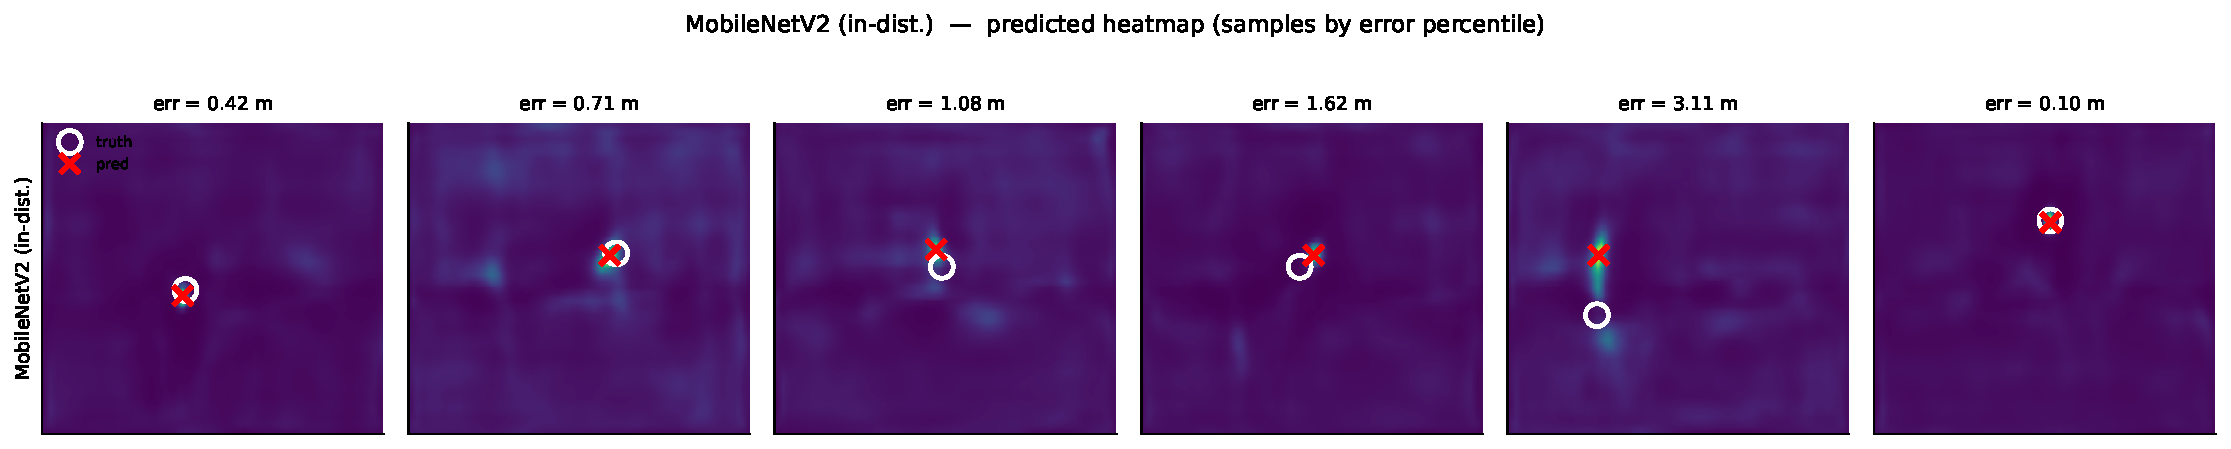
\includegraphics[width=\linewidth]{heatmaps_mobilenet_fig10b.pdf}
\caption{In-distribution qualitative predictions --- MobileNetV2.}
\label{fig:app:hm_mobilenet}
\end{figure}

\begin{figure}[H]
\centering
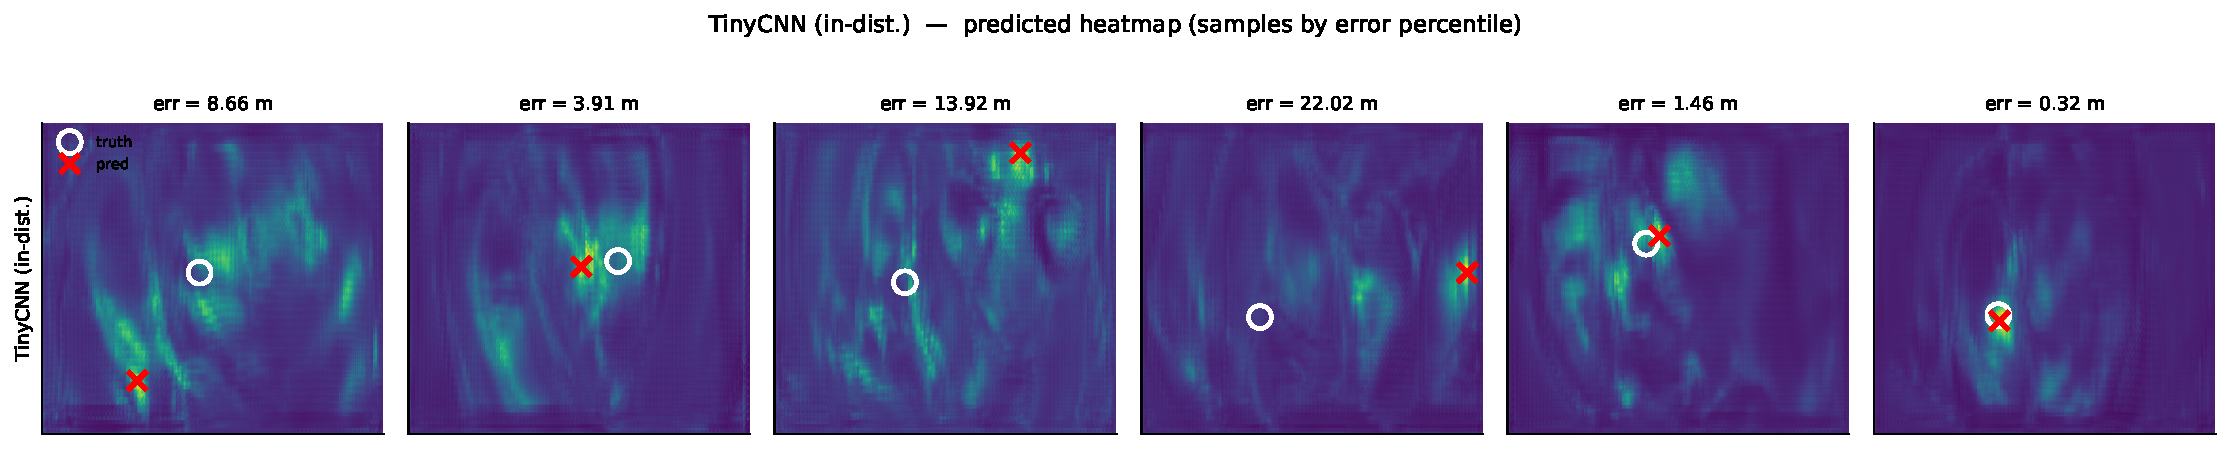
\includegraphics[width=\linewidth]{heatmaps_tinycnn_fig10b.pdf}
\caption{In-distribution qualitative predictions --- TinyCNN. The broader, less-peaked heatmaps are
consistent with the model's high median error.}
\label{fig:app:hm_tinycnn}
\end{figure}

\begin{figure}[H]
\centering
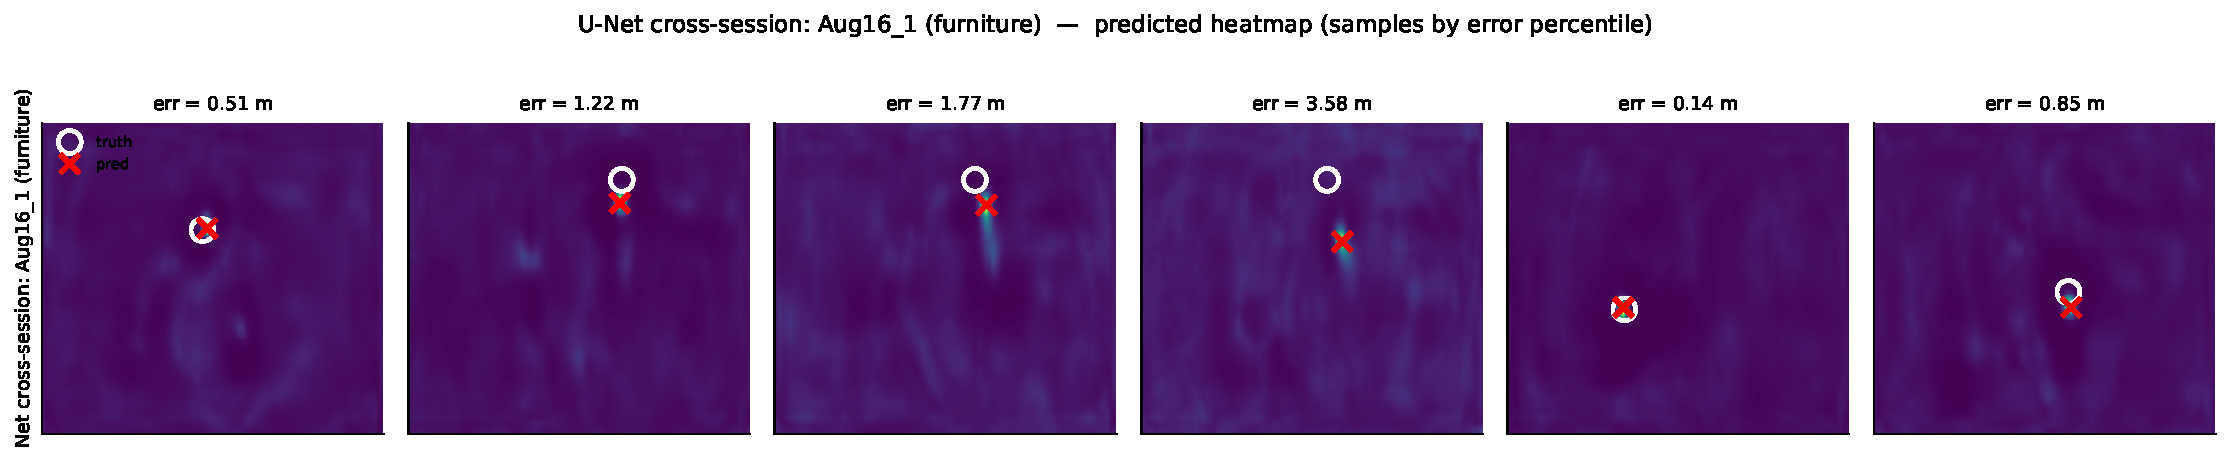
\includegraphics[width=\linewidth]{heatmaps_unet_cross_env2.pdf}
\caption{Cross-session qualitative predictions --- MobileNetV2-UNet on Aug16\_1 (furniture).}
\label{fig:app:hm_cross2}
\end{figure}

\begin{figure}[H]
\centering
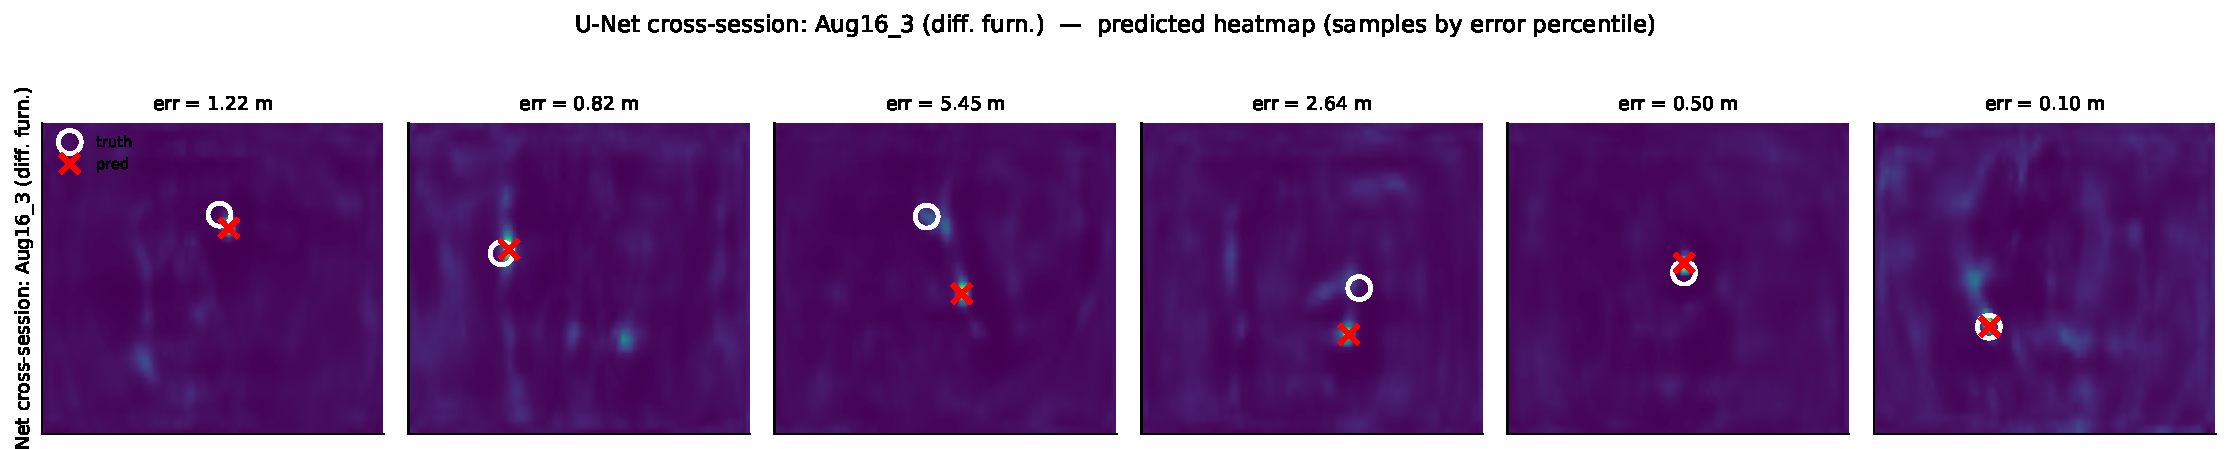
\includegraphics[width=\linewidth]{heatmaps_unet_cross_env3.pdf}
\caption{Cross-session qualitative predictions --- MobileNetV2-UNet on Aug16\_3 (different furniture).}
\label{fig:app:hm_cross3}
\end{figure}
